% ================================================================
% The Retrieve and Connect version of latex/starters/targeted/KS3/numberSense/numberSenseStarters.tex
%
% This is the same deck as the one above, made by renaming the titles in it.
% Every slide that was a numbered starter is now titled
% "Retrieve and Connect", and the word is renamed wherever else a title
% used it. Nothing outside a title has been changed.
%
%   made from           latex/starters/targeted/KS3/numberSense/numberSenseStarters.tex
%   retitling rules     version 1
%
% Please don't edit this file. It is written again from the one it was
% made from whenever that changes, so an edit here would be lost - edit
% that file instead and this one follows.
% ================================================================
\documentclass{beamer}
\usepackage{tikz}
\usetikzlibrary{calc}
\usepackage{xcolor}
\usepackage{multicol}
\usepackage{amsmath}
\usepackage{amssymb}

% ================================================================
% Answer-overlay helpers
% ================================================================
\newcommand{\ablank}[1]{%
  \alt<2>{\textcolor{red}{#1}}{\underline{\phantom{#1}}}%
}
\newcommand{\ashow}[1]{\uncover<2->{\textcolor{red}{\small #1}}}
\newcommand{\ashowq}[1]{\alt<2->{\textcolor{red}{\small #1}}{?}}

% Answers drawn straight on to a TikZ diagram, revealed on overlay 2 like \ashow.
% Space is reserved on overlay 1, so the diagram does not move between slides.
\usetikzlibrary{overlay-beamer-styles}
\tikzset{
  ans/.style     = {red, thick, visible on=<2->},
  ansfill/.style = {red!15, visible on=<2->},
  anslab/.style  = {red, font=\tiny, visible on=<2->},
}

% Used by the worked solutions rather than by this deck, so that each worked
% solution is first a question with room to write in and then the answer.
\newlength{\aworkpad}
\setlength{\aworkpad}{8mm}
\newcommand{\awork}[1]{%
  \par\vspace{\aworkpad}%
  \uncover<2->{#1}%
  \par\vspace{\aworkpad}%
}

% Tighter list spacing, so eight questions fit on one frame.
\newcommand{\qtight}{%
  \setlength{\itemsep}{0pt}\setlength{\parskip}{0pt}\setlength{\parsep}{0pt}%
  \setlength{\topsep}{0pt}\setlength{\partopsep}{0pt}%
}
\setlength{\columnsep}{8pt}

\title{Number Sense: Retrieve and Connects}
\author{}
\date{}

\begin{document}

\frame{\titlepage}

%------------------------------------------------
% STARTER 1: Number Lines and Place Value
%------------------------------------------------
\begin{frame}{Retrieve and Connect}

\vspace{-2.5em}

\begin{columns}[T]

\column{0.30\textwidth}
\begin{center}
\vspace{3em}
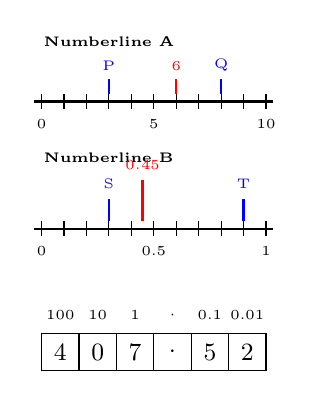
\begin{tikzpicture}[scale=0.95]

% --- Line A: 0 to 10, ticks every 1 ---
\node[font=\tiny\bfseries, anchor=west] at (-0.1,4.6) {Numberline A};
\draw[thick] (-0.1,3.8) -- (3.1,3.8);
\foreach \x in {0,0.3,0.6,0.9,1.2,1.5,1.8,2.1,2.4,2.7,3}
  \draw (\x,3.7) -- (\x,3.9);
\foreach \x/\lab in {0/0,1.5/5,3/10} \node[font=\tiny] at (\x,3.5) {\lab};
% Given points: P at 3, Q at 8. Kept low, so they stay clear of the Line A heading.
\draw[blue, thick] (0.9,3.9) -- (0.9,4.1);
\node[blue, font=\tiny] at (0.9,4.28) {P};
\draw[blue, thick] (2.4,3.9) -- (2.4,4.1);
\node[blue, font=\tiny] at (2.4,4.28) {Q};
% --- Q3 answer: 6 marked on Line A ---
\draw[ans] (1.8,3.9) -- (1.8,4.1);
\node[anslab] at (1.8,4.28) {$6$};

% --- Numberline B: 0 to 1 in tenths ---
\node[font=\tiny\bfseries, anchor=west] at (-0.1,3.05) {Numberline B};
\draw[thick] (-0.1,2.1) -- (3.1,2.1);
\foreach \x in {0,0.3,0.6,0.9,1.2,1.5,1.8,2.1,2.4,2.7,3}
  \draw (\x,2.0) -- (\x,2.2);
\foreach \x/\lab in {0/0,1.5/0.5,3/1} \node[font=\tiny] at (\x,1.8) {\lab};
% Given points: S at 0.3, T at 0.9
\draw[blue, thick] (0.9,2.2) -- (0.9,2.5);
\node[blue, font=\tiny] at (0.9,2.7) {S};
\draw[blue, thick] (2.7,2.2) -- (2.7,2.5);
\node[blue, font=\tiny] at (2.7,2.7) {T};
% --- Q3 answer: 0.45 marked on Line B, raised clear of the blue S label ---
\draw[ans] (1.35,2.2) -- (1.35,2.75);
\node[anslab] at (1.35,2.95) {$0.45$};

% --- Place value chart for 407.52 ---

\foreach \i/\head/\digit in {0/100/4,1/10/0,2/1/7,3/{$\cdot$}/{$\cdot$},4/0.1/5,5/0.01/2} {
  \draw ({0.5*\i},0.2) rectangle ({0.5*\i+0.5},0.7);
  \node[font=\tiny] at ({0.5*\i+0.25},0.95) {\head};
  \node[font=\small] at ({0.5*\i+0.25},0.45) {\digit};
}

\end{tikzpicture}
\end{center}

\column{0.70\textwidth}

\small
\begin{multicols}{2}
\begin{enumerate}\qtight

  \item On numberline A what numbers are marked by  $P$ and $Q$? \ashow{$3$ and $8$}

  \item On numberline B what numbers are marked by  $S$ and $T$? \ashow{$0.3$ and $0.9$}

  \item Mark $6$ on Line~A and $0.45$ on Line~B.

  \item Sam says $P=4$, as it is the $4$th mark. What has he done wrong? \ashow{Counted marks, not steps: $P=3$}
  \columnbreak

  \item The chart shows $407.52$. What is the $4$ worth? And the $5$? \ashow{$400$ and $0.5$}


  \item Work out $407.52\times 10$ and $407.52\div 10$. \ashow{$4075.2$ and $40.752$}

  \item A numberline goes $3.6$ to $3.7$ in $10$ equal steps. What is $3$ steps along from $3.6$? \ashow{$3.63$}

  \item Use $7$, $5$, $4$, $2$ and a decimal point to make the largest number less than $100$. \ashow{$75.42$}

\end{enumerate}
\end{multicols}

\end{columns}

\end{frame}

%------------------------------------------------
% STARTER 2: Inequality Symbols and Ordering Decimals
%------------------------------------------------
\begin{frame}{Retrieve and Connect: Inequality Symbols \& Ordering Decimals}

\vspace{-2.5em}

\begin{columns}[T]

\column{0.30\textwidth}
\begin{center}
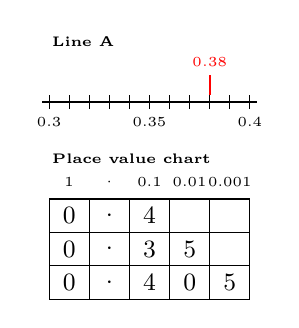
\begin{tikzpicture}[scale=0.85]

% --- Line A: 0.3 to 0.4 in hundredths ---
\node[font=\tiny\bfseries, anchor=west] at (-0.1,3.5) {Line A};
\draw[thick] (-0.1,2.6) -- (3.1,2.6);
\foreach \x in {0,0.3,0.6,0.9,1.2,1.5,1.8,2.1,2.4,2.7,3}
  \draw (\x,2.5) -- (\x,2.7);
\foreach \x/\lab in {0/0.3,1.5/0.35,3/0.4} \node[font=\tiny] at (\x,2.3) {\lab};
% --- Q5 answer: 0.38 marked ---
\draw[ans] (2.4,2.7) -- (2.4,3.0);
\node[anslab] at (2.4,3.2) {$0.38$};

% --- Place value chart: 0.4, 0.35, 0.405 ---
\node[font=\tiny\bfseries, anchor=west] at (-0.1,1.75) {Place value chart};
\foreach \i/\head in {0/1,1/{$\cdot$},2/0.1,3/0.01,4/0.001}
  \node[font=\tiny] at ({0.6*\i+0.3},1.4) {\head};
\foreach \j in {0,1,2} {
  \foreach \i in {0,1,2,3,4}
    \draw ({0.6*\i},{-0.5*\j+1.15}) rectangle ({0.6*\i+0.6},{-0.5*\j+0.65});
}
% row 1: 0.4
\foreach \i/\d in {0/0,1/{$\cdot$},2/4} \node[font=\small] at ({0.6*\i+0.3},0.9) {\d};
% row 2: 0.35
\foreach \i/\d in {0/0,1/{$\cdot$},2/3,3/5} \node[font=\small] at ({0.6*\i+0.3},0.4) {\d};
% row 3: 0.405
\foreach \i/\d in {0/0,1/{$\cdot$},2/4,3/0,4/5} \node[font=\small] at ({0.6*\i+0.3},-0.1) {\d};

\end{tikzpicture}
\end{center}

\column{0.70\textwidth}

\small
\begin{multicols}{2}
\begin{enumerate}\qtight

  \item Fill in $<$ or $>$: $7 \mathrel{\text{\ashowq{$<$}}} 12$, $30 \mathrel{\text{\ashowq{$>$}}} 3$

  \item In $0.405$, what is the $4$ worth? \ashow{$4$ tenths, $0.4$}

  \item Chart: which is bigger, $0.4$ or $0.35$? Why? \ashow{$0.4$: $4$ tenths beats $3$}

  \item Fill in $<$, $>$ or $=$: $0.4 \mathrel{\text{\ashowq{$=$}}} 0.40$, $0.6 \mathrel{\text{\ashowq{$>$}}} 0.06$

  \item Mark $0.38$ on Line A. Is it nearer $0.3$ or $0.4$? \ashow{nearer $0.4$}

  \columnbreak

  \item Order, smallest first: $0.5$, $0.45$, $0.405$, $0.54$ \ashow{($0.405$, $0.45$, $0.5$, $0.54$)}

  \item (Extension) True or false: more digits \emph{after} the point means bigger? Give an example. \ashow{False: $0.9>0.1234$}

  \item (Challenge) Alfie says $0.45>0.5$ as $45>5$. Explain his mistake, then write a decimal between $0.4$ and $0.405$. \ashow{$0.5$ has $5$ tenths; e.g.\ $0.402$}

\end{enumerate}
\end{multicols}

\end{columns}

\end{frame}

%------------------------------------------------
% STARTER 3: Negative Numbers
%------------------------------------------------
\begin{frame}{Retrieve and Connect: Ordering Negative Numbers}

\vspace{-2.5em}

\begin{columns}[T]

\column{0.30\textwidth}
\begin{center}
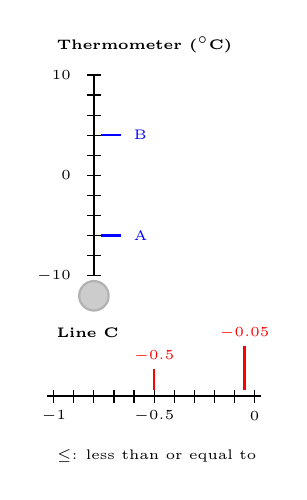
\begin{tikzpicture}[scale=0.85]

% --- Thermometer: -10 to 10, one tick every 2 degrees, only -10/0/10 labelled ---
\node[font=\tiny\bfseries, anchor=west] at (-0.1,3.45) {Thermometer ($^\circ$C)};
\draw[thick] (0.6,0) -- (0.6,3);
\foreach \y in {0,0.3,0.6,0.9,1.2,1.5,1.8,2.1,2.4,2.7,3}
  \draw (0.5,\y) -- (0.7,\y);
\foreach \y/\lab in {0/{$-10$},1.5/{$0$},3/{$10$}}
  \node[font=\tiny, anchor=east] at (0.4,\y) {\lab};
\fill[gray!40] (0.6,-0.3) circle (0.22);
\draw[gray!60, thick] (0.6,-0.3) circle (0.22);
% Given readings: A at -6, B at 4 (both sit exactly on a tick)
\draw[blue, thick] (0.7,0.6) -- (1.0,0.6);
\node[blue, font=\tiny, anchor=west] at (1.05,0.6) {A};
\draw[blue, thick] (0.7,2.1) -- (1.0,2.1);
\node[blue, font=\tiny, anchor=west] at (1.05,2.1) {B};

% --- Line C: -1 to 0 in tenths ---
\node[font=\tiny\bfseries, anchor=west] at (-0.1,-0.85) {Line C};
\draw[thick] (-0.1,-1.8) -- (3.1,-1.8);
\foreach \x in {0,0.3,0.6,0.9,1.2,1.5,1.8,2.1,2.4,2.7,3}
  \draw (\x,-1.9) -- (\x,-1.7);
\foreach \x/\lab in {0/{$-1$},1.5/{$-0.5$},3/{$0$}} \node[font=\tiny] at (\x,-2.1) {\lab};
% Reminder for the challenge question, which is the deck's only use of a weak inequality
\node[font=\tiny, anchor=west] at (-0.1,-2.7) {$\leq$: less than or equal to};
% --- Q5 answers: -0.5 and -0.05 marked on Line C, at different heights ---
\draw[ans] (1.5,-1.7) -- (1.5,-1.4);
\node[anslab] at (1.5,-1.2) {$-0.5$};
\draw[ans] (2.85,-1.7) -- (2.85,-1.05);
\node[anslab] at (2.85,-0.85) {$-0.05$};

\end{tikzpicture}
\end{center}

\column{0.70\textwidth}

\small
\begin{multicols}{2}
\begin{enumerate}\qtight

  \item Which is colder, $4\,^\circ$C or $-4\,^\circ$C? \ashow{$-4\,^\circ$C}

  \item What is each mark on the thermometer worth? Write the temperatures at A and B. \ashow{$2\,^\circ$C per mark; A $=-6$, B $=4$}

  \item Which is colder, $-3$ or $-8$? Fill in: $-3 \mathrel{\text{\ashowq{$>$}}} -8$ \ashow{($-8$ is colder)}

  \item Order, smallest first: $-2$, $5$, $-7$, $0$, $-1$ \ashow{($-7,-2,-1,0,5$)}

  \columnbreak

  \item Mark $-0.5$ and $-0.05$ on Line C. Which is larger? \ashow{$-0.05$}

  \item Fill in $<$ or $>$: $-4.5 \mathrel{\text{\ashowq{$<$}}} -4.05$, $-0.3 \mathrel{\text{\ashowq{$<$}}} 0.03$

  \item (Extension) Order, smallest first: $-0.08$, $0.7$, $-0.8$, $-0.75$ \ashow{($-0.8$, $-0.75$, $-0.08$, $0.7$)}

  \item (Challenge) List the integers $n$: $-3\leq n<2$. Write a number between $-0.5$ and $-0.4$. \ashow{$-3,-2,-1,0,1$; e.g.\ $-0.45$}

\end{enumerate}
\end{multicols}

\end{columns}

\end{frame}

%------------------------------------------------
% STARTER 4: Rounding Integers
%------------------------------------------------
\begin{frame}{Retrieve and Connect: Rounding Integers}

\vspace{-2.5em}

\begin{columns}[T]

\column{0.30\textwidth}
\begin{center}
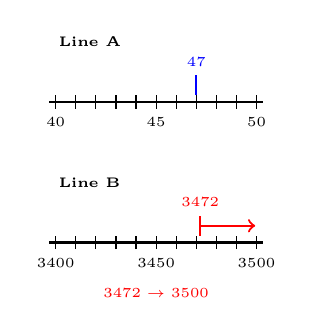
\begin{tikzpicture}[scale=0.85]

% --- Line A: 40 to 50, ticks every 1 ---
\node[font=\tiny\bfseries, anchor=west] at (-0.1,3.5) {Line A};
\draw[thick] (-0.1,2.6) -- (3.1,2.6);
\foreach \x in {0,0.3,0.6,0.9,1.2,1.5,1.8,2.1,2.4,2.7,3}
  \draw (\x,2.5) -- (\x,2.7);
\foreach \x/\lab in {0/40,1.5/45,3/50} \node[font=\tiny] at (\x,2.3) {\lab};
% Given point: 47
\draw[blue, thick] (2.1,2.7) -- (2.1,3.0);
\node[blue, font=\tiny] at (2.1,3.2) {$47$};

% --- Line B: 3400 to 3500, ticks every 10 ---
\node[font=\tiny\bfseries, anchor=west] at (-0.1,1.4) {Line B};
\draw[thick] (-0.1,0.5) -- (3.1,0.5);
\foreach \x in {0,0.3,0.6,0.9,1.2,1.5,1.8,2.1,2.4,2.7,3}
  \draw (\x,0.4) -- (\x,0.6);
\foreach \x/\lab in {0/3400,1.5/3450,3/3500} \node[font=\tiny] at (\x,0.2) {\lab};
% --- Q4 answers: 3472 marked, with an arrow to the nearer end ---
\draw[ans] (2.16,0.6) -- (2.16,0.9);
\node[anslab] at (2.16,1.1) {$3472$};
\draw[ans, ->] (2.16,0.75) -- (2.98,0.75);
\node[anslab] at (1.5,-0.25) {$3472 \to 3500$};

\end{tikzpicture}
\end{center}

\column{0.70\textwidth}

\small
\begin{multicols}{2}
\begin{enumerate}\qtight

  \item Fill in $<$ or $>$: $-6 \mathrel{\text{\ashowq{$<$}}} -2$

  \item Line A: is $47$ nearer $40$ or $50$? Round it to the nearest $10$. \ashow{nearer $50$, so $50$}

  \item Round to the nearest $10$: $32$, $85$ \ashow{($30$ and $90$)}

  \item Mark $3472$ on Line B, then round it to the nearest $100$.

  \item Round $3472$ to the nearest $10$; to the nearest $1000$. \ashow{$3470$ and $3000$}

  \columnbreak

  \item Round $4950$ to the nearest $100$. \ashow{$5000$}

  \item (Extension) Zoe rounds $8449$ to the nearest $100$: $8449\to 8450\to 8500$. What is her mistake? \ashow{Rounded twice: only the tens digit $4$ counts, so $8400$}

  \item (Challenge) A number rounds to $250$ to the nearest $10$. Smallest it could be? Largest? \ashow{$245$ and $254$}

\end{enumerate}
\end{multicols}

\end{columns}

\end{frame}

%------------------------------------------------
% STARTER 5: Rounding Decimals, Recurring and Irrational
%------------------------------------------------
\begin{frame}{Retrieve and Connect: Rounding Decimals \& Never-Ending Decimals}

\vspace{-2.5em}

\begin{columns}[T]

\column{0.30\textwidth}
\begin{center}
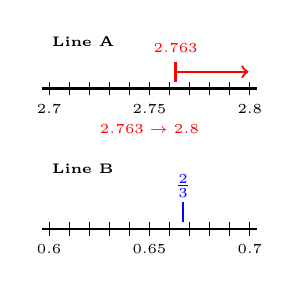
\begin{tikzpicture}[scale=0.85]

% --- Line A: 2.7 to 2.8 in hundredths ---
% Heading sits at 3.3 rather than 3.5: this frame's title is two lines' worth of
% width and the diagram column otherwise crowds it.
\node[font=\tiny\bfseries, anchor=west] at (-0.1,3.3) {Line A};
\draw[thick] (-0.1,2.6) -- (3.1,2.6);
\foreach \x in {0,0.3,0.6,0.9,1.2,1.5,1.8,2.1,2.4,2.7,3}
  \draw (\x,2.5) -- (\x,2.7);
\foreach \x/\lab in {0/2.7,1.5/2.75,3/2.8} \node[font=\tiny] at (\x,2.3) {\lab};
% (the Line A heading sits low here, to keep clear of the frame title)
% --- Q3 answers: 2.763 marked, with an arrow to the nearer end ---
\draw[ans] (1.89,2.7) -- (1.89,3.0);
\node[anslab] at (1.89,3.2) {$2.763$};
\draw[ans, ->] (1.89,2.85) -- (2.98,2.85);
\node[anslab] at (1.5,2.0) {$2.763 \to 2.8$};

% --- Line B: 0.6 to 0.7 in hundredths, with 2/3 shown ---
\node[font=\tiny\bfseries, anchor=west] at (-0.1,1.4) {Line B};
\draw[thick] (-0.1,0.5) -- (3.1,0.5);
\foreach \x in {0,0.3,0.6,0.9,1.2,1.5,1.8,2.1,2.4,2.7,3}
  \draw (\x,0.4) -- (\x,0.6);
\foreach \x/\lab in {0/0.6,1.5/0.65,3/0.7} \node[font=\tiny] at (\x,0.2) {\lab};
% Given point: 2/3 = 0.6666...
\draw[blue, thick] (2.0,0.6) -- (2.0,0.9);
\node[blue, font=\scriptsize] at (2.0,1.15) {$\tfrac{2}{3}$};

\end{tikzpicture}

\vspace{0.4em}
{\scriptsize
\begin{tabular}{@{}l@{}}
\textbf{Never-ending decimals} \\[0.15em]
$\frac{2}{3} = 0.6666\ldots = 0.\dot{6}$ \\
$\frac{1}{7} = 0.142857142857\ldots$ \\
$\pi = 3.14159265\ldots$ \\
$\sqrt{2} = 1.41421356\ldots$ \\
$0.1010010001\ldots$
\end{tabular}}
\end{center}

\column{0.70\textwidth}

\small
\begin{multicols}{2}
\begin{enumerate}\qtight

  \item Round $4738$ to the nearest $100$. \ashow{$4700$}

  \item Round to the nearest whole number: $4.6$, $12.348$ \ashow{($5$ and $12$)}

  \item Mark $2.763$ on Line A. Round it to $1$ decimal place (d.p.).

  \item Round to $1$ d.p.: $4.62$, $0.95$. Why is $0.95$ not $1$? \ashow{$4.6$, $1.0$ --- $1$ d.p.\ needs one decimal digit}

  \item Round $12.348$ to $2$ d.p., then to $1$ d.p. Why not $12.4$? \ashow{$12.35$, $12.3$ --- never round twice}

  \columnbreak

  \item Line B shows $\frac{2}{3}=0.\dot{6}$. Round it to $1$ d.p.\ and $2$ d.p. \ashow{$0.7$ and $0.67$}

  \item (Extension) Write $\frac{1}{3}$ in dot notation, then round $\frac{1}{7}$ to $3$ d.p. \ashow{$0.\dot{3}$ and $0.143$}

  \item (Challenge) Which listed decimals never settle into a repeating block? Can one still be a fraction? \ashow{$\pi$, $\sqrt{2}$, $0.101001\ldots$; yes: $0.\dot{3}=\frac13$}

\end{enumerate}
\end{multicols}

\end{columns}

\end{frame}

\end{document}